% ŠABLONA PRO PSANÍ ZÁVĚREČNÉ STUDIJNÍ PRÁCE
%%%%%%%%%%%%%%%%%%%%%%%%%%%%%%%%%%%%%%%%%%%%
% Autor: Jakub Dokulil (kubadokulil99@gmail.com)
% Tato šablona byla vytvořena tak, aby pomocí ní mohli v systému LaTeX soutěžící sázet své práce a zároveň odpovídala požadavkům na formátování vyplývajícím z wordové šablony umístěné na webu soc.cz.
%
\documentclass[12pt, a4paper, twoside, openright]{report}

\usepackage[T1]{fontenc}
\usepackage[utf8]{inputenc}
\usepackage[czech]{babel}
\usepackage{lmodern}

\usepackage{tikz}

%% Nutné balíčky a nastavení
%%%%%%%%%%%%%%%%%%%%%%%%%%%%

%% Proměnné
\newcommand\obor{INFORMAČNÍ TECHNOLOGIE} %% -- napiš číslo a název tvého oboru
\newcommand\kodOboru{18-20-M/01} %% -- napiš číslo a název tvého oboru
\newcommand\zamereni{se zaměřením na počítačové sítě a programování} %% -- napiš číslo a název tvého oboru
\newcommand\skola{Střední škola průmyslová a umělecká, Opava} %% vyplň název školy
\newcommand\trida{IT4} %% vyplň jméno svého konzultanta
\newcommand\jmenoAutora{Daniel Holeš}  %% vyplň své jméno
\newcommand\skolniRok{2024/25} %% vyplň rok
\newcommand\datumOdevzdani{1. 1. 2025} %% vyplň rok
\newcommand\nazevPrace{Repetito - Mobilní aplikace pro efektivní učení metodou spaced repetition} %% vyplň název své práce

\title{\nazevPrace} %% -- Název tvé práce
\author{\jmenoAutora} %% -- tvé jméno
\date{\datumOdevzdani} %% -- rok, kdy píšeš SOČku

\usepackage[top=2.5cm, bottom=2.5cm, left=3.5cm, right=1.5cm]{geometry} %% nastaví okraje, left -- vnitřní okraj, right -- vnější okraj

\usepackage[czech]{babel} %% balík babel pro sazbu v češtině
\usepackage[utf8]{inputenc} %% balíky pro kódování textu
\usepackage[T1]{fontenc}
\usepackage{cmap} %% balíček zajišťující, že vytvořené PDF bude prohledávatelné a kopírovatelné
\usepackage{lmodern}  % Přidáno pro lepší podporu českých znaků

\usepackage{graphicx} %% balík pro vkládání obrázků

\usepackage{subcaption} %% balíček pro vkládání podobrázků

\usepackage{hyperref} %% balíček, který v PDF vytváří odkazy

\linespread{1.25} %% řádkování
\setlength{\parskip}{0.5em} %% odsazení mezi odstavci


\usepackage[pagestyles]{titlesec} %% balíček pro úpravu stylu kapitol a sekcí

% Nastavení formátování nadpisů
\titleformat{\chapter}[hang]
  {\rmfamily\bfseries\Large}  % Zmenšeno z \LARGE na \Large
  {\thechapter}
  {1em}
  {\MakeUppercase}

\titleformat{\section}[hang]
  {\rmfamily\bfseries\large}  % Zmenšeno z \Large na \large
  {\thesection}
  {1em}
  {}

\titleformat{\subsection}[hang]
  {\rmfamily\bfseries\normalsize}  % Zmenšeno z \large na \normalsize
  {\thesubsection}
  {1em}
  {}

% Nastavení mezer před a za nadpisy
\titlespacing*{\chapter}{0pt}{-30pt}{8pt}  % Zmenšeno z 20pt na 8pt
\titlespacing*{\section}{0pt}{12pt}{4pt}   % Zmenšeno z 20pt/10pt na 12pt/4pt
\titlespacing*{\subsection}{0pt}{12pt}{4pt} % Zmenšeno z 20pt/10pt na 12pt/4pt

% Nastavení formátování pro nečíslované nadpisy
\titleformat{name=\chapter,numberless}[hang]
  {\rmfamily\bfseries\Large}
  {}
  {0pt}
  {\MakeUppercase}

\titleformat{name=\section,numberless}[hang]
  {\rmfamily\bfseries\large}  % Zmenšeno z \Large na \large
  {}
  {0pt}
  {}

% Nastavení mezer pro nečíslované nadpisy
\titlespacing*{name=\chapter,numberless}{0pt}{0pt}{8pt}  % Změněno z -30pt na 0pt pro první mezeru
\titlespacing*{name=\section,numberless}{0pt}{12pt}{4pt}   % Zmenšeno z 15pt/5pt na 12pt/4pt

% Nastavení fontu pro obsah
\renewcommand{\cfttoctitlefont}{\rmfamily\LARGE\bfseries}
\renewcommand{\cftchapfont}{\rmfamily\bfseries}
\renewcommand{\cftsecfont}{\rmfamily}
\renewcommand{\cftsubsecfont}{\rmfamily}

% Nastavení číslování pro obsah
\renewcommand{\cftchappresnum}{\rmfamily\bfseries}
\renewcommand{\cftsecpresnum}{\rmfamily}
\renewcommand{\cftsubsecpresnum}{\rmfamily}

\usepackage{tocloft} % Balíček pro přizpůsobení vzhledu obsahu
\setlength{\cftbeforechapskip}{10pt}  % Větší rozestup pro kapitoly
\setlength{\cftbeforesecskip}{3pt}   % Menší rozestup pro sekce

% Nastavení odsazení a formátování obsahu
\cftsetindents{chapter}{0em}{2.5em}
\cftsetindents{section}{2.5em}{3em}
\cftsetindents{subsection}{5.5em}{3.7em}
\renewcommand{\cftdotsep}{2} % Hustota teček
\renewcommand{\cftchapleader}{\cftdotfill{\cftdotsep}} % Tečky i pro kapitoly

\setcounter{secnumdepth}{2}
\setcounter{tocdepth}{2}
\usepackage{fancyhdr}
\pagestyle{fancy}
\renewcommand{\headrulewidth}{0.025pt}

\usepackage{booktabs}

\usepackage{url}

%% Balíčky co se můžou hodit :) 
%%%%%%%%%%%%%%%%%%%%%%%%%%%%%%%

\usepackage{pdfpages} %% Balíček umožňující vkládat stránky z PDF souborů, 

\usepackage{upgreek} %% Balíček pro sazbu stojatých řeckých písmen, třeba u jednotky mikrometr. Například stojaté mí: \upmu, stojaté pí: \uppi

\usepackage{amsmath}    %% Balíčky amsmath a amsfonts 
\usepackage{amsfonts}   %% pro sazbu matematických symbolů
\usepackage{esint}     %% pro sazbu různých integrálů (např \oiint)
\usepackage{mathrsfs}
\usepackage{helvet} % Helvet font
\usepackage{mathptmx} % Times New Roman
\usepackage{Oswald} % Oswald font


%% makra pro sazbu matematiky
\newcommand{\dif}{\mathrm{d}} %% makro pro sazbu diferenciálu, místo toho
%% abych musel psát '\mathrm{d}' mi stačí napsat '\dif' což je mnohem 
%% kratší a mohu si tak usnadnit práci

\usepackage{listings}
\usepackage{xcolor}

\renewcommand{\lstlistingname}{Kód}% Listing -> Algorithm
\renewcommand{\lstlistlistingname}{Seznam programových kódů}% List of Listings -> List of Algorithms

%% Definice 
\lstdefinelanguage{JavaScript}{
	morekeywords=[1]{break, continue, delete, else, for, function, if, in,
		new, return, this, typeof, var, void, while, with},
	% Literals, primitive types, and reference types.
	morekeywords=[2]{false, null, true, boolean, number, undefined,
		Array, Boolean, Date, Math, Number, String, Object},
	% Built-ins.
	morekeywords=[3]{eval, parseInt, parseFloat, escape, unescape},
	sensitive,
	morecomment=[s]{/*}{*/},
	morecomment=[l]//,
	morecomment=[s]{/**}{*/}, % JavaDoc style comments
	morestring=[b]',
	morestring=[b]"
}[keywords, comments, strings]


\lstdefinelanguage[ECMAScript2015]{JavaScript}[]{JavaScript}{
	morekeywords=[1]{await, async, case, catch, class, const, default, do,
		enum, export, extends, finally, from, implements, import, instanceof,
		let, static, super, switch, throw, try},
	morestring=[b]` % Interpolation strings.
}

\lstalias[]{ES6}[ECMAScript2015]{JavaScript}

% Nastavení barev
% Requires package: color.
\definecolor{mediumgray}{rgb}{0.3, 0.4, 0.4}
\definecolor{mediumblue}{rgb}{0.0, 0.0, 0.8}
\definecolor{forestgreen}{rgb}{0.13, 0.55, 0.13}
\definecolor{darkviolet}{rgb}{0.58, 0.0, 0.83}
\definecolor{royalblue}{rgb}{0.25, 0.41, 0.88}
\definecolor{crimson}{rgb}{0.86, 0.8, 0.24}

% Nastavení pro Python
\lstdefinestyle{Python}{
	language=Python,
	backgroundcolor=\color{white},
	basicstyle=\ttfamily,
	breakatwhitespace=false,
	breaklines=false,
	captionpos=b,
	columns=fullflexible,
	commentstyle=\color{mediumgray}\upshape,
	emph={},
	emphstyle=\color{crimson},
	extendedchars=true,  % requires inputenc
	fontadjust=true,
	frame=single,
	identifierstyle=\color{black},
	keepspaces=true,
	keywordstyle=\color{mediumblue},
	keywordstyle={[2]\color{darkviolet}},
	keywordstyle={[3]\color{royalblue}},
	literate=%
	{á}{{\'a}}1 {č}{{\v{c}}}1 {ď}{{\v{d}}}1 {é}{{\'e}}1 {ě}{{\v{e}}}1
	{í}{{\'i}}1 {ň}{{\v{n}}}1 {ó}{{\'o}}1 {ř}{{\v{r}}}1 {š}{{\v{s}}}1
	{ť}{{\v{t}}}1 {ú}{{\'u}}1 {ů}{{\r{u}}}1 {ý}{{\'y}}1 {ž}{{\v{z}}}1,		
	numbers=left,
	numbersep=5pt,
	numberstyle=\tiny\color{black},
	rulecolor=\color{black},
	showlines=true,
	showspaces=false,
	showstringspaces=false,
	showtabs=false,
	stringstyle=\color{forestgreen},
	tabsize=2,
	title=\lstname,
	upquote=true  % requires textcomp	
}


\lstdefinestyle{JSES6Base}{
	backgroundcolor=\color{white},
	basicstyle=\ttfamily,
	breakatwhitespace=false,
	breaklines=false,
	captionpos=b,
	columns=fullflexible,
	commentstyle=\color{mediumgray}\upshape,
	emph={},
	emphstyle=\color{crimson},
	extendedchars=true,  % requires inputenc
	fontadjust=true,
	frame=single,
	identifierstyle=\color{black},
	keepspaces=true,
	keywordstyle=\color{mediumblue},
	keywordstyle={[2]\color{darkviolet}},
	keywordstyle={[3]\color{royalblue}},
 literate=%
{á}{{\'a}}1 {č}{{\v{c}}}1 {ď}{{\v{d}}}1 {é}{{\'e}}1 {ě}{{\v{e}}}1
{í}{{\'i}}1 {ň}{{\v{n}}}1 {ó}{{\'o}}1 {ř}{{\v{r}}}1 {š}{{\v{s}}}1
{ť}{{\v{t}}}1 {ú}{{\'u}}1 {ů}{{\r{u}}}1 {ý}{{\'y}}1 {ž}{{\v{z}}}1,		
	numbers=left,
	numbersep=5pt,
	numberstyle=\tiny\color{black},
	rulecolor=\color{black},
	showlines=true,
	showspaces=false,
	showstringspaces=false,
	showtabs=false,
	stringstyle=\color{forestgreen},
	tabsize=2,
	title=\lstname,
	upquote=true  % requires textcomp
}

\lstdefinestyle{JavaScript}{
	language=JavaScript,
	style=JSES6Base,
}
\lstdefinestyle{ES6}{
	language=ES6,
	style=JSES6Base
}


%% Bordel pro práci - můžeš smáznout :) 
%%%%%%%%%%%%%%%%%%%

\usepackage{lipsum} %% balíček který píše lipsum (nesmyslný text, který se používá pro kontrolu typografie)

%% Začátek dokumentu
%%%%%%%%%%%%%%%%%%%%
\begin{document}
	
	\pagestyle{empty}
	\pagenumbering{arabic}
	
	\cleardoublepage

%% Titulní stránka s informacemi
%%%%%%%%%%%%%%%%%%%%%%%%%%%%%%%%%%%%%%%%
	
	{\fontfamily{phv}\selectfont
		%% Logo školy
		\begin{figure}[h]
			\centering
			
\includegraphics[width=0.6\linewidth]{image/logo-skoly.png}
		\end{figure}
		
		
		%% Hlavička práce a její název (viz proměnná \nazev prace)
		%% \sffamily %%% bezpatkové písmo - sans serif
		{\bfseries %%% písmo na stránce je tučně
			\begin{center}
				\vspace{0.025 \textheight}
				\LARGE{ZÁVĚREČNÁ STUDIJNÍ PRÁCE}\\
				\large{dokumentace}\\
				\vspace{0.075 \textheight}
				\LARGE {\nazevPrace}\\
			\end{center}  
		}%%%
		
		\begin{figure}[h]
			\centering
			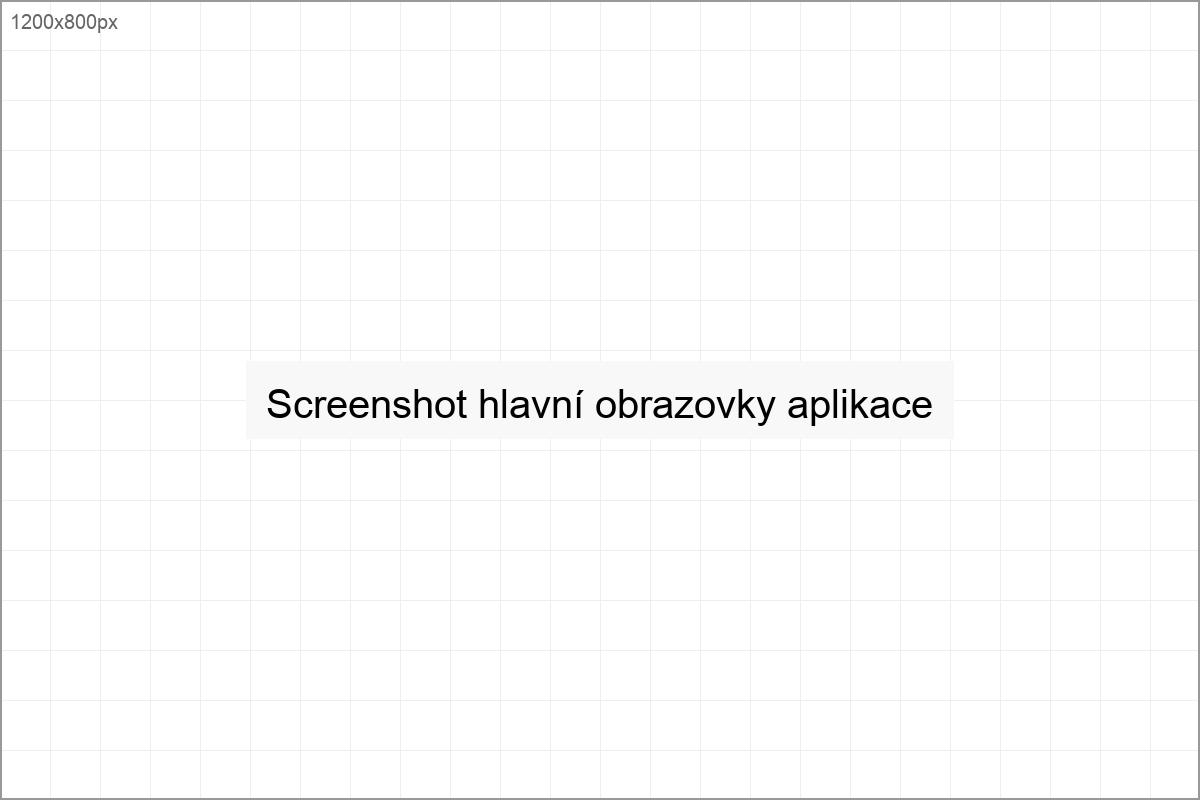
\includegraphics[width=0.8\linewidth]{image/screenshot-main.jpg}
			\label{fig:main-screen}
		\end{figure}
		
		\vspace{0.02 \textheight}
		\begin{table}[h!]
			\begin{tabular}{ll}
				\textbf{Autor:} & \jmenoAutora\\ 
				\textbf{Obor:} & \kodOboru { } \obor\\
				\textbf{} & \zamereni\\
				\textbf{Třída:} & \trida\\
				\textbf{Školní rok:} & \skolniRok\\
			\end{tabular}
			
		\end{table}		
	}
	
\cleardoublepage %% Zalomení dvojstránky
	
	\tableofcontents
	\cleardoublepage

%% Stránka obsahující poděkování a prohlášení
%%%%%%%%%%%%%%%%%%%%%%%%%%%%%%%%%%%%%%%%%%%%%%%%%%%%%%%%

%% Poděkování - nepovinné
%%%%%%%%%%%%%%%%%%%%%%%%%%%%
	
	\noindent{\large{\bfseries{Poděkování}\\}}
	\noindent Děkuji panu učiteli Mgr. Markovi Lucnemu a Ing. Petru Grussmanovi za rady při vytváření tohoto projektu.
	
	\vspace*{0.7\textheight} %% Vertikální mezeru je možné upravit

%% Prohlášení - povinné
%%%%%%%%%%%%%%%%%%%%%%%%%%%%
	\noindent{\large{\bfseries{Prohlášení}\\}}  %% uprav si koncovky podle toho na jaký rod se cítíš, vypadá to pak lépe :) 
	\noindent{Prohlašuji, že jsem závěrečnou práci vypracoval samostatně a uvedl veškeré použité 
		informační zdroje.\\}
	\noindent{Souhlasím, aby tato studijní práce byla použita k výukovým a prezentačním účelům na Střední průmyslové a umělecké škole v Opavě, Praskova 399/8.}
	\vfill
	\noindent{V Opavě \datumOdevzdani\\}
	\noindent
	\begin{minipage}{\linewidth}
		\hspace{9.5cm} 
		\begin{tabular}{@{}p{6cm}@{}}
			\dotfill \\
			Podpis autora
		\end{tabular}
	\end{minipage}
	
	\cleardoublepage %% Zalomení dvojstránky

%% Stránka obsahující abstrakt (anotaci)
%%%%%%%%%%%%%%%%%%%%%%%%%%%%%%%%%%%%%%%%%%%%%%%%%%%%%%%%	
%% Abstrakt v češtině
%%%%%%%%%%%%%%%%%%%%%%%%%%%%
	\noindent{\Large{\bfseries{Abstrakt}\\}}
	\addcontentsline{toc}{chapter}{Abstrakt}
	Mobilní aplikace Repetito je vzdělávací nástroj využívající metodu spaced repetition pro efektivní učení a zapamatování informací. Aplikace je implementována pomocí frameworku Flutter s využitím Riverpod pro správu stavu a Supabase jako backend řešení. Dokumentace popisuje architekturu aplikace, implementační detaily a způsoby řešení. Důraz je kladen na offline funkcionalitu a synchronizaci dat mezi zařízeními.

	\vspace{18pt}
	\noindent{\large{\bfseries{Klíčová slova}}}

	\noindent Flutter, Riverpod, Supabase, spaced repetition, mobilní aplikace, vzdělávání

	\vspace{18pt}
	\noindent{\Large{\bfseries{Abstract}\\}}
	The Repetito mobile application is an educational tool that uses the spaced repetition method for effective learning and information retention. The application is implemented using the Flutter framework with Riverpod for state management and Supabase as a backend solution. The documentation describes the application architecture, implementation details and solutions. Emphasis is placed on offline functionality and data synchronization between devices.

	\vspace{18pt}
	\noindent{\large{\bfseries{Keywords}}}

	\noindent Flutter, Riverpod, Supabase, spaced repetition, mobile application, education

	\chapter*{Seznam použitých zkratek}
	\addcontentsline{toc}{chapter}{Seznam použitých zkratek}
	\begin{tabular}{ll}
		API & Application Programming Interface,\\
		CRUD & Create, Read, Update, Delete,\\
		HTTP & Hypertext Transfer Protocol,\\
		JSON & JavaScript Object Notation,\\
		REST & Representational State Transfer,\\
		SQL & Structured Query Language,\\
		UI & User Interface,\\
		UX & User Experience.\\
	\end{tabular}

%% Definice příkazu pro podnadpisy v úvodu
\newcommand{\introsubheading}[1]{%
  {\noindent\textbf{\normalsize #1}\vspace{1pt}\par}%
}

\chapter*{ÚVOD}
\addcontentsline{toc}{chapter}{Úvod}

\introsubheading{Představení projektu}
V současné době, kdy se mobilní aplikace staly nedílnou součástí našeho života, roste i potřeba efektivních nástrojů pro vzdělávání. Tradiční metody učení často nevedou k dlouhodobému zapamatování informací, zatímco vědecky podložený přístup spaced repetition využívá přirozených mechanismů lidské paměti. Projekt Repetito vznikl s cílem vytvořit moderní vzdělávací aplikaci, která kombinuje tento osvědčený princip učení s možnostmi současných technologií. Aplikace řeší běžné nedostatky existujících řešení, jako je absence efektivních metod pro dlouhodobé zapamatování a omezená možnost práce offline.

\introsubheading{Motivace}
Hlavní motivací pro vytvoření aplikace Repetito byla osobní zkušenost s nedostatky současných vzdělávacích aplikací. Většina dostupných řešení buď nenabízí efektivní metody pro dlouhodobé zapamatování, nebo postrádá možnost práce v offline režimu. Současně roste potřeba efektivního učení v době, kdy množství informací, které potřebujeme vstřebat, neustále narůstá. Aplikace Repetito vznikla s cílem poskytnout uživatelům nástroj, který nejen implementuje vědecky podložené metody učení, ale také nabízí moderní a intuitivní uživatelské rozhraní spolu s pokročilými funkcemi jako je synchronizace mezi zařízeními.

\introsubheading{Cíle projektu}
Hlavním cílem této práce je vytvořit mobilní aplikaci pro efektivní učení pomocí metody spaced repetition. Aplikace musí umožňovat vytváření a správu učebních sad, implementovat algoritmus spaced repetition pro optimální plánování opakování a poskytovat plnohodnotnou offline funkcionalitu. Důležitým aspektem je také synchronizace dat mezi zařízeními a intuitivní uživatelské rozhraní, které uživatelům usnadní pravidelné učení.

\introsubheading{Struktura práce}
Práce je rozdělena do několika hlavních částí. První kapitola se zabývá teoretickou ��ástí, která popisuje principy učení, paměti a metodu spaced repetition. Druhá kapitola popisuje frontend aplikace včetně použitého frameworku Flutter a architektury aplikace. Třetí kapitola se věnuje využitým technologiím jako Riverpod a Supabase. Čtvrtá kapitola detailně rozebírá způsoby řešení a použité postupy při implementaci. Pátá kapitola shrnuje dosažené výsledky a práci uzavírá závěrečné zhodnocení projektu s výhledem do budoucna.

\chapter{Teoretická část}
	\section{Principy učení a paměti}
	Lidská paměť funguje na základě komplexních neurologických procesů. Při učení dochází k vytváření a posilování synaptických spojení v mozku. Efektivita zapamatování je ovlivněna mnoha faktory, včetně časování opakování, kontextu učení a emocionálního stavu. Výzkumy ukazují, že pravidelné opakování v optimálních intervalech výrazně zvyšuje dlouhodobou retenci informací.

	\section{Metoda Spaced Repetition}
	Spaced repetition (učení s rozestupy) je technika učení založená na opakování informací v optimálních časových intervalech. Tato metoda vychází z poznatků kognitivní psychologie a výzkumů lidské paměti. Základním principem je, že čím lépe si pamatujeme určitou informaci, tím del��í může být interval do dalšího opakování.

	\subsection{Historie a výzkum}
	Historie metody spaced repetition sahá do konce 19. stolet��, kdy německý psycholog Hermann Ebbinghaus provedl prokopnický experimenty v oblasti lidské paměti. Jeho výzkum, publikovaný v roce 1885 v díle "Über das Gedächtnis"(O paměti), položil základy pro pochopení procesu zapomínání a učení.

	Ebbinghausovy experimenty byly unikátní svou metodologií:
	\begin{itemize}
		\item Použití nesmyslných slabik pro eliminaci vlivu předchozích znalostí.
		\item Systematické měření schopnosti vybavit si informace v různých časových intervalech.
		\item Kvantifikace procesu zapomínání pomocí matematických funkcí.
	\end{itemize}

	Na Ebbinghausovu práci navázali v průběhu 20. století další vzkumníci:
	\begin{itemize}
		\item Cecil Alec Mace (1932) - první systematický výzkum efektivity rozloženého učení.
		\item Paul Pimsleur (1967) - vytvoření exponenciálního systému intervalů pro jazykové učení.
		\item Sebastian Leitner (1970) - vývoj systému učebních kartiček s různými intervaly opakování.
	\end{itemize}

	\subsection{Ebbinghausova křivka zapomínání}
	Ebbinghausova křivka zapomínání je matematický model popisující, jak rychle zapomínáme nově naučené informace. Křivka ukazuje, že:
	\begin{itemize}
		\item Největší ztráta informací nastává v prvních hodinách po učen��.
		\item Po 24 hodinách si pamatujeme pouze 40\% naučeného.
		\item Po týdnu klesá retence na přibližně 20\%.
		\item Opakování v správných intervalech výrazně zpomaluje proces zapomínání.
	\end{itemize}

	Matematicky lze křivku zapomínání vyjádřit vztahem:
	\begin{equation}
		R = e^{-t/S}
	\end{equation}
	kde:
	\begin{itemize}
		\item R je retence (míra zapamatování)
		\item t je čas od učení
		\item S je síla paměti
	\end{itemize}

	\section{Analýza existujících řešení}
	V současné době existuje několik populárních aplikací pro spaced repetition učení, každá s vlastními specifickými přístupy a funkcionalitami:

	\begin{itemize}
		\item Anki
		\begin{itemize}
			\item Nejrozšířenější open-source řešení.
			\item Robustní synchronizační systém.
			\item Komplexní možnosti přizpůsobení.
			\item Složitější uživatelské rozhraní.
			\item Omezená podpora mobilních zařízení.
		\end{itemize}

		\item Quizlet
		\begin{itemize}
			\item Populární mezi studenty.
			\item Intuitivní uživatelské rozhraní.
			\item Rozsáhlá komunita sdílejících obsah.
			\item Omezené možnosti spaced repetition.
			\item Vyžaduje prmiové předplatné pro pokročilé funkce.
		\end{itemize}

		\item Memrise
		\begin{itemize}
			\item Zaměření především na jazykové učení.
			\item Propracovaný gamifikační systém.
			\item Multimediální obsah.
			\item Omezená možnost vlastního obsahu.
			\item Závislost na internetovém připojení.
		\end{itemize}
	\end{itemize}

	\subsection{Srovnání funkcionalit}
	Pro lepší přehled o možnostech jednotlivých aplikací byla vytvořena srovnávací tabulka klíčových funkcionalit:

	\begin{table}[h]
		\centering
		\begin{tabular}{lccc}
			\toprule
			\textbf{Funkcionalita} & \textbf{Anki} & \textbf{Quizlet} & \textbf{Memrise} \\
			\midrule
			Offline režim & Ano & Částečně & Ne \\
			Synchronizace & Ano & Ano & Ano \\
			Vlastní obsah & Ano & Ano & Omezený \\
			Sdílení obsahu & Ano & Ano & Ne \\
			Statistiky učení & Pokročilé & Základní & Základní \\
			Gamifikace & Ne & Částečně & Ano \\
			Mobilní aplikace & Omezená & Ano & Ano \\
			Zdarma & Ano & Částečně & Částečně \\
			\bottomrule
		\end{tabular}
		\caption{Srovnání funkcionalit existujících řešení}
		\label{tab:functionality-comparison}
	\end{table}

	Z tabulky je patrné, že každá aplikace má své silné a slabé stránky. Zatímco Anki vyniká v pokročilých funkcích a statistikách, postrádá moderní uživatelské rozhraní a gamifikační prvky. Quizlet nabízí dobrou rovnováhu mezi funkcionalitou a použitelností, ale mnoho pokročilých funkcí je dostupných pouze v placené verzi. Memrise má propracovaný systém gamifikace, ale je omezen především na jazykové učení a vyžaduje stálé připojení k internetu.

\chapter{Použité technologie}
	\section{Flutter \& Dart}
	Základem aplikace je programovací jazyk Dart ve verzi 3.0.

	Klíčové vlastnosti Dart:
	\begin{itemize}
		\item Robustní podpora null safety
		\item Silný typový systém
		\item AOT kompilace pro produkci
		\item JIT kompilace pro vývoj
		\item Pokročilé asynchronní programování
	\end{itemize}

	Flutter představuje moderní open-source UI framework od společnosti Google, který umožňuje vývoj nativních aplikací pro různé platformy z jedné codebáze.

	Klíčové vlastnosti frameworku:
	\begin{itemize}
		\item Hot Reload pro okamžité zobrazení změn v kódu
		\item Bohatá sada předpřipravených Material a Cupertino widgetů
		\item Vysoký výkon díky kompilaci do nativního kódu
		\item Jednotná codebáze pro všechny podporované platformy
		\item Deklarativní p��ístup k tvorbě UI
	\end{itemize}

	\section{Riverpod}
	Pro správu stavu aplikace jsem zvolil framework Riverpod.

	Klíčové funkce Riverpod:
	\begin{itemize}
		\item Typově bezpečné providers
		\item Integrovaná dependency injection
		\item Podpora reaktivního programování
		\item Automatická správa životního cyklu
		\item Snadná testovatelnost
	\end{itemize}

	Implementované typy providerů:
	\begin{itemize}
		\item AsyncNotifierProvider pro asynchronní operace
		\item NotifierProvider pro synchronní stav
		\item StreamProvider pro reaktivní datové toky
		\item StateProvider pro jednoduchý lokální stav
		\item FamilyProvider pro parametrizované providery
	\end{itemize}

	\section{Supabase}
	Jako backend řešení jsem implementoval Supabase.

	\begin{figure}[h]
		\centering
		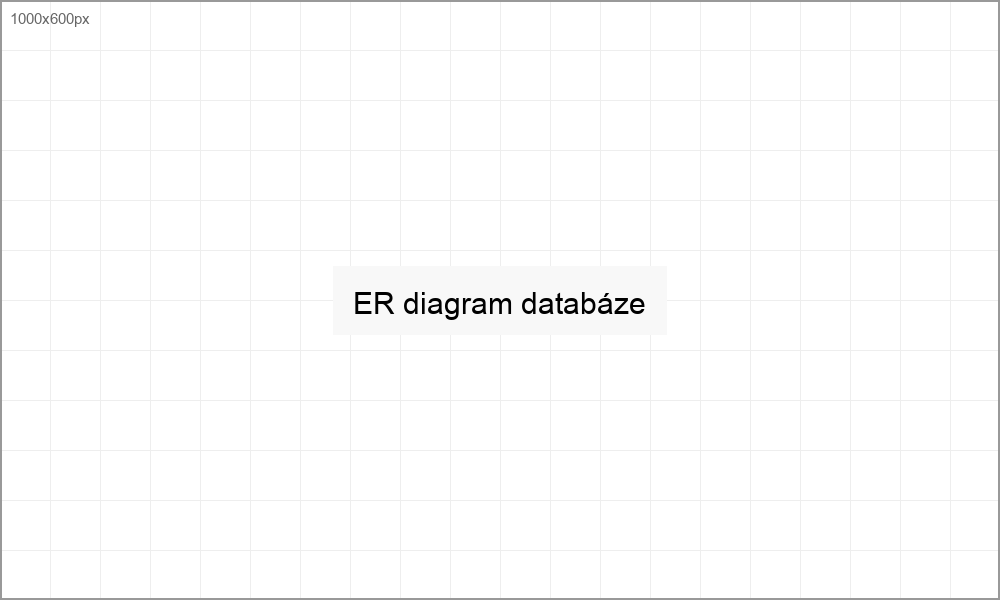
\includegraphics[width=0.8\linewidth]{image/diagram-databaze.png}
		\caption{ER diagram databáze}
		\label{fig:database}
	\end{figure}

	Klíčové funkce Supabase:
	\begin{itemize}
		\item PostgreSQL databáze
		\item Realtime subscriptions
		\item Row Level Security
		\item REST a GraphQL API
		\item Vestavná autentizace
	\end{itemize}

	\section{GoRouter}
	Navigační systém aplikace je postaven na knihovně GoRouter.

	Implementované funkce:
	\begin{itemize}
		\item Deklarativní přístup k routingu
		\item Deep linking podpora
		\item Nested routes
		\item Path parametry
		\item Přehledná správa navigačního stavu
	\end{itemize}

	\section{Freezed}
	Pro generování kódu využíváme nástroj Freezed.

	Hlavní přínosy:
	\begin{itemize}
		\item Generování immutable tříd
		\item Podpora union types
		\item JSON serializace
		\item Pattern matching
		\item Automatické generování equals a hashCode
	\end{itemize}

\chapter{Architektura aplikace}
	\section{Celková architektura}
	Aplikaci jsem postavil na principech Clean Architecture, což zajišťuje jasné oddělení business logiky od uživatelského rozhraní.

	\begin{figure}[h]
		\centering
		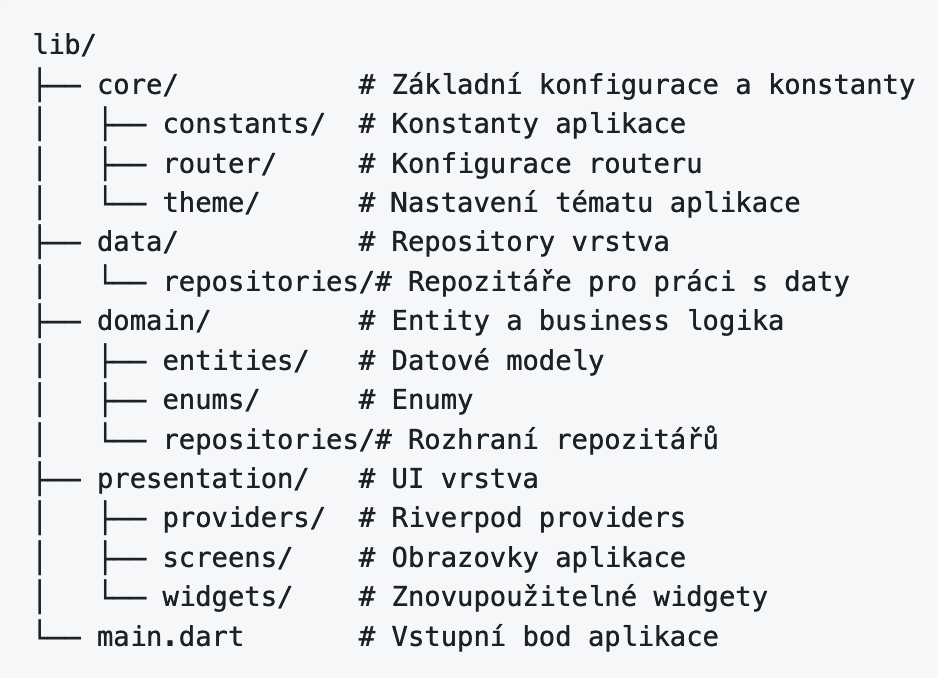
\includegraphics[width=0.8\linewidth]{image/diagram-architektura.png}
		\caption{Architektura aplikace}
		\label{fig:architecture}
	\end{figure}

	Hlavní architektonické principy:
	\begin{itemize}
		\item Lepší testovatelnost jednotlivých komponent
		\item Snadnější údržba a rozšiřitelnost kódu
		\item Jasná separace zodpovědností
		\item Konzistentní terminologie v celém projektu
		\item Škálovatelnost aplikace
	\end{itemize}

	\section{Datový model}
	Pro reprezentaci dat v aplikaci jsem použil immutabilní třídy generované pomocí balíčku Freezed. Tento přístup zajišťuje typovou bezpečnost a snadnou serializaci dat.

	\begin{lstlisting}[style=Python, caption=Definice datových modelů]
// Balíček karet pro učení
@freezed
class DeckEntity with _$DeckEntity {
  const factory DeckEntity({
    required String id,          // Unikátní identifikátor
    required String name,        // Název balíčku
    required String description, // Popis balíčku
    required DateTime createdAt, // Datum vytvoření
    required DateTime updatedAt, // Datum poslední změny
    @Default(false) bool isDeleted,  // Příznak smazání
  }) = _DeckEntity;

  // Deserializace z JSON
  factory DeckEntity.fromJson(Map<String, dynamic> json) => 
      _$DeckEntityFromJson(json);
}

// Jednotlivá učební karta
@freezed
class CardEntity with _$CardEntity {
  const factory CardEntity({
    required String id,          // Unikátní identifikátor
    required String deckId,      // Odkaz na balíček
    required String front,       // Přední strana (otázka)
    required String back,        // Zadní strana (odpověď)
    required DateTime createdAt, // Datum vytvoření
    required DateTime updatedAt, // Datum poslední změny
    @Default(false) bool isDeleted,  // Příznak smazán��
  }) = _CardEntity;

  // Deserializace z JSON
  factory CardEntity.fromJson(Map<String, dynamic> json) => 
      _$CardEntityFromJson(json);
}
	\end{lstlisting}

\chapter{Implementace}
	\section{Frontend implementace}
	\subsection{Uživatelské rozhraní}
	Design uživatelského rozhraní následuje principy Material Design 3. Návrh rozhraní začal vytvořením wireframů klíčových obrazovek:

	\begin{figure}[h]
		\centering
		\begin{subfigure}[b]{0.48\textwidth}
			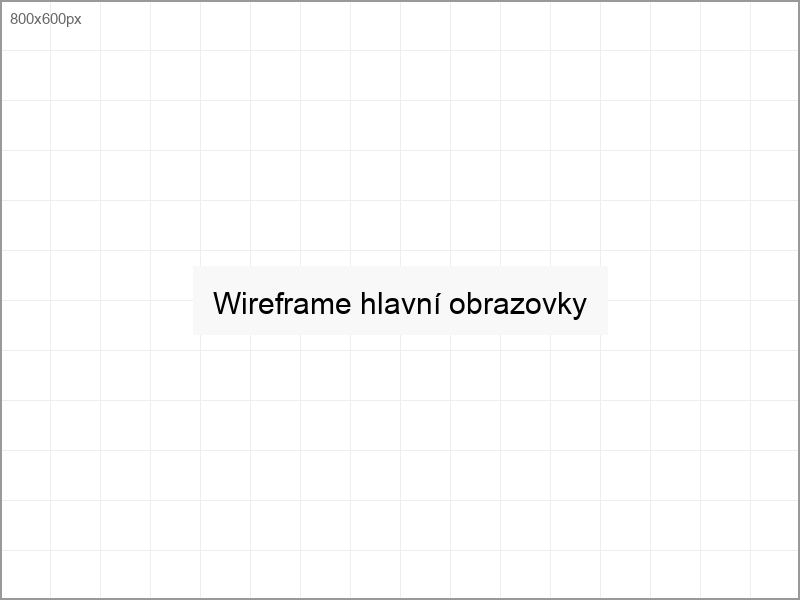
\includegraphics[width=\linewidth]{image/wireframe-main.png}
			\caption{Wireframe hlavní obrazovky}
			\label{fig:wireframe-main}
		\end{subfigure}
		\hfill
		\begin{subfigure}[b]{0.48\textwidth}
			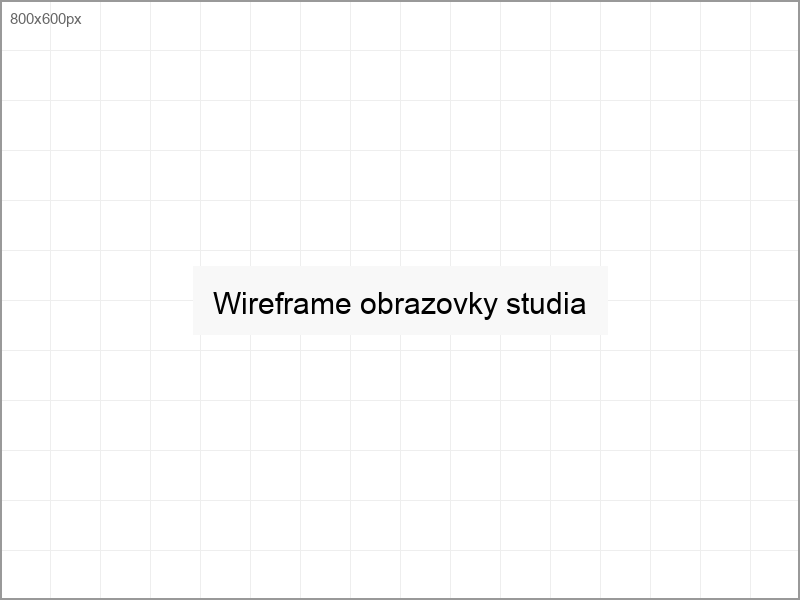
\includegraphics[width=\linewidth]{image/wireframe-study.png}
			\caption{Wireframe obrazovky studia}
			\label{fig:wireframe-study}
		\end{subfigure}
		\caption{Wireframy klíčových obrazovek}
		\label{fig:wireframes}
	\end{figure}

	Na základě wireframů byla implementována finální podoba aplikace:

	\begin{figure}[h]
		\centering
		\begin{subfigure}[b]{0.48\textwidth}
			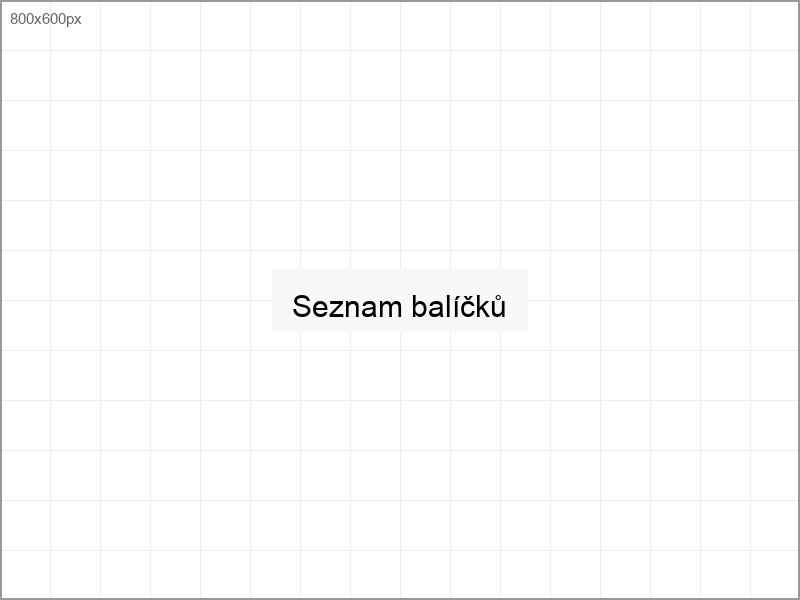
\includegraphics[width=\linewidth]{image/screen-deck-list.png}
			\caption{Seznam balíčků}
			\label{fig:screen-decks}
		\end{subfigure}
		\hfill
		\begin{subfigure}[b]{0.48\textwidth}
			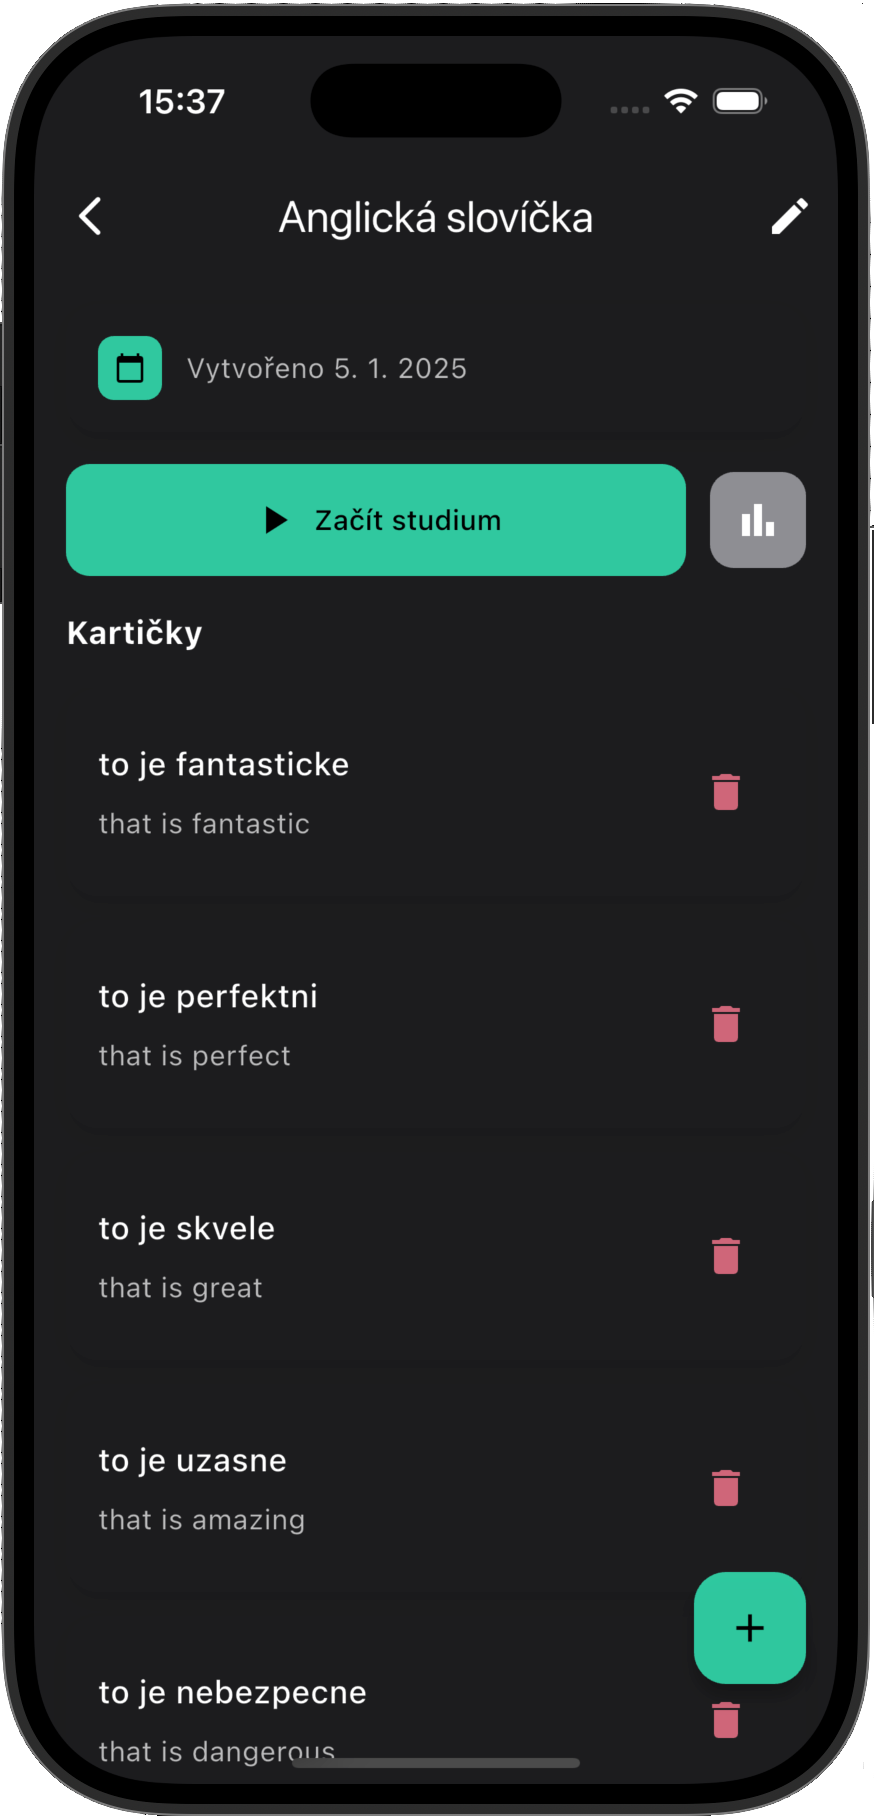
\includegraphics[width=\linewidth]{image/screen-deck-detail.png}
			\caption{Detail balíčku}
			\label{fig:screen-detail}
		\end{subfigure}
		\caption{Hlavní obrazovky aplikace}
		\label{fig:screens}
	\end{figure}

	\begin{figure}[h]
		\centering
		\begin{subfigure}[b]{0.48\textwidth}
			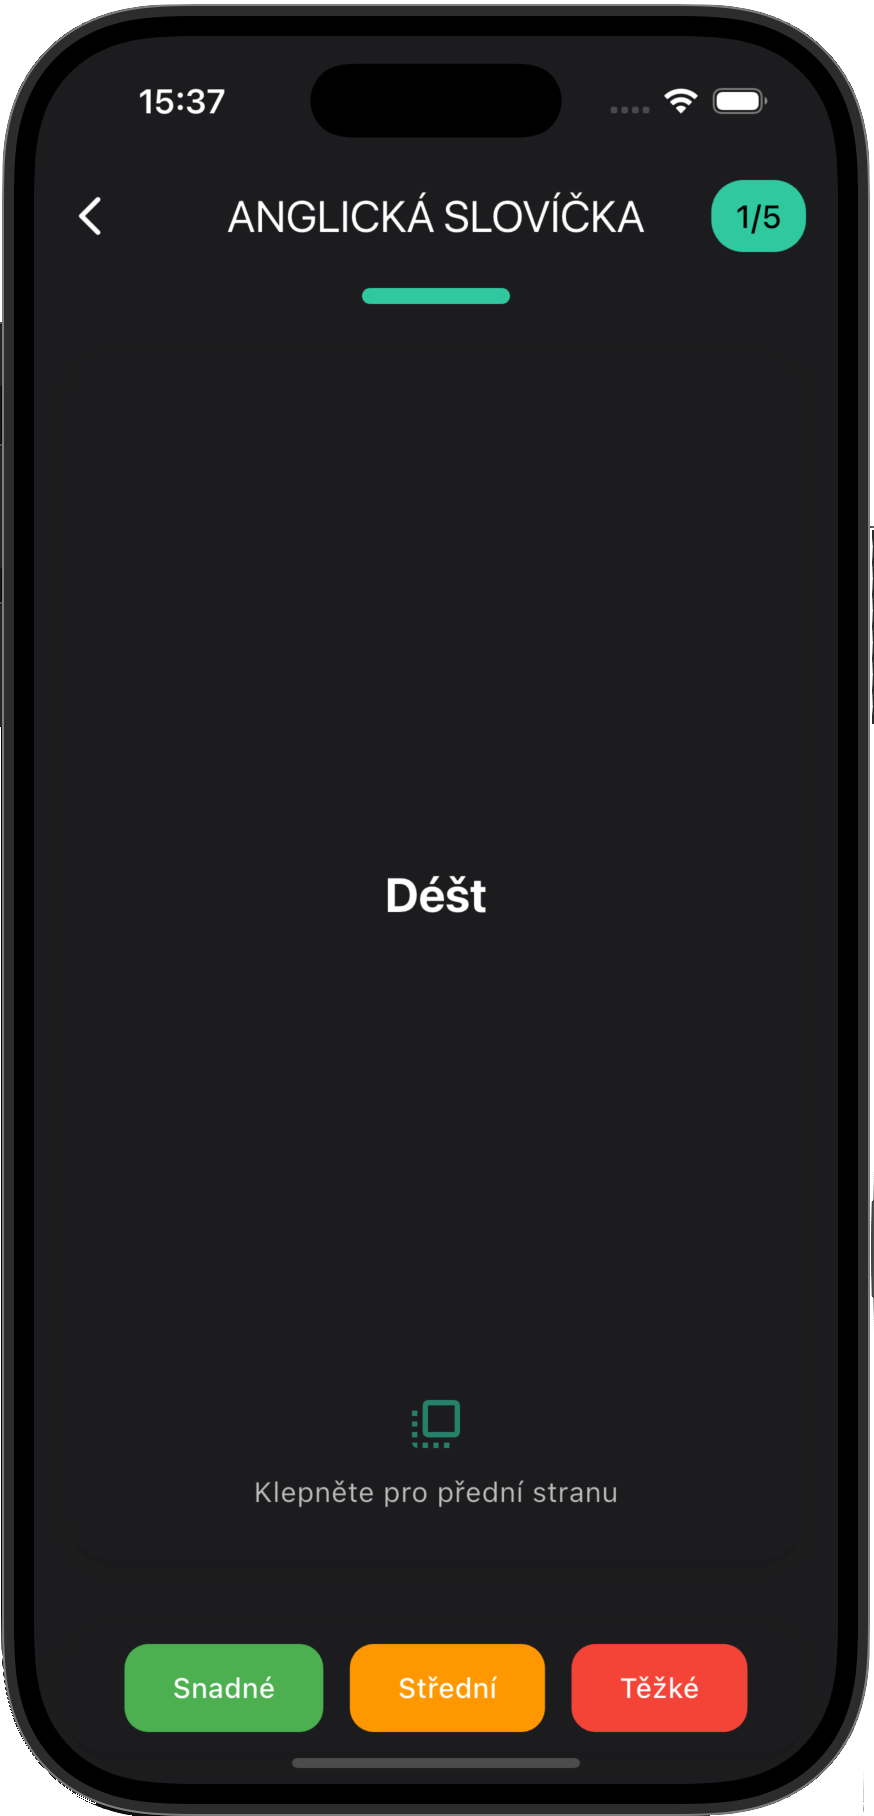
\includegraphics[width=\linewidth]{image/screen-study.png}
			\caption{Obrazovka studia}
			\label{fig:screen-study}
		\end{subfigure}
		\hfill
		\begin{subfigure}[b]{0.48\textwidth}
			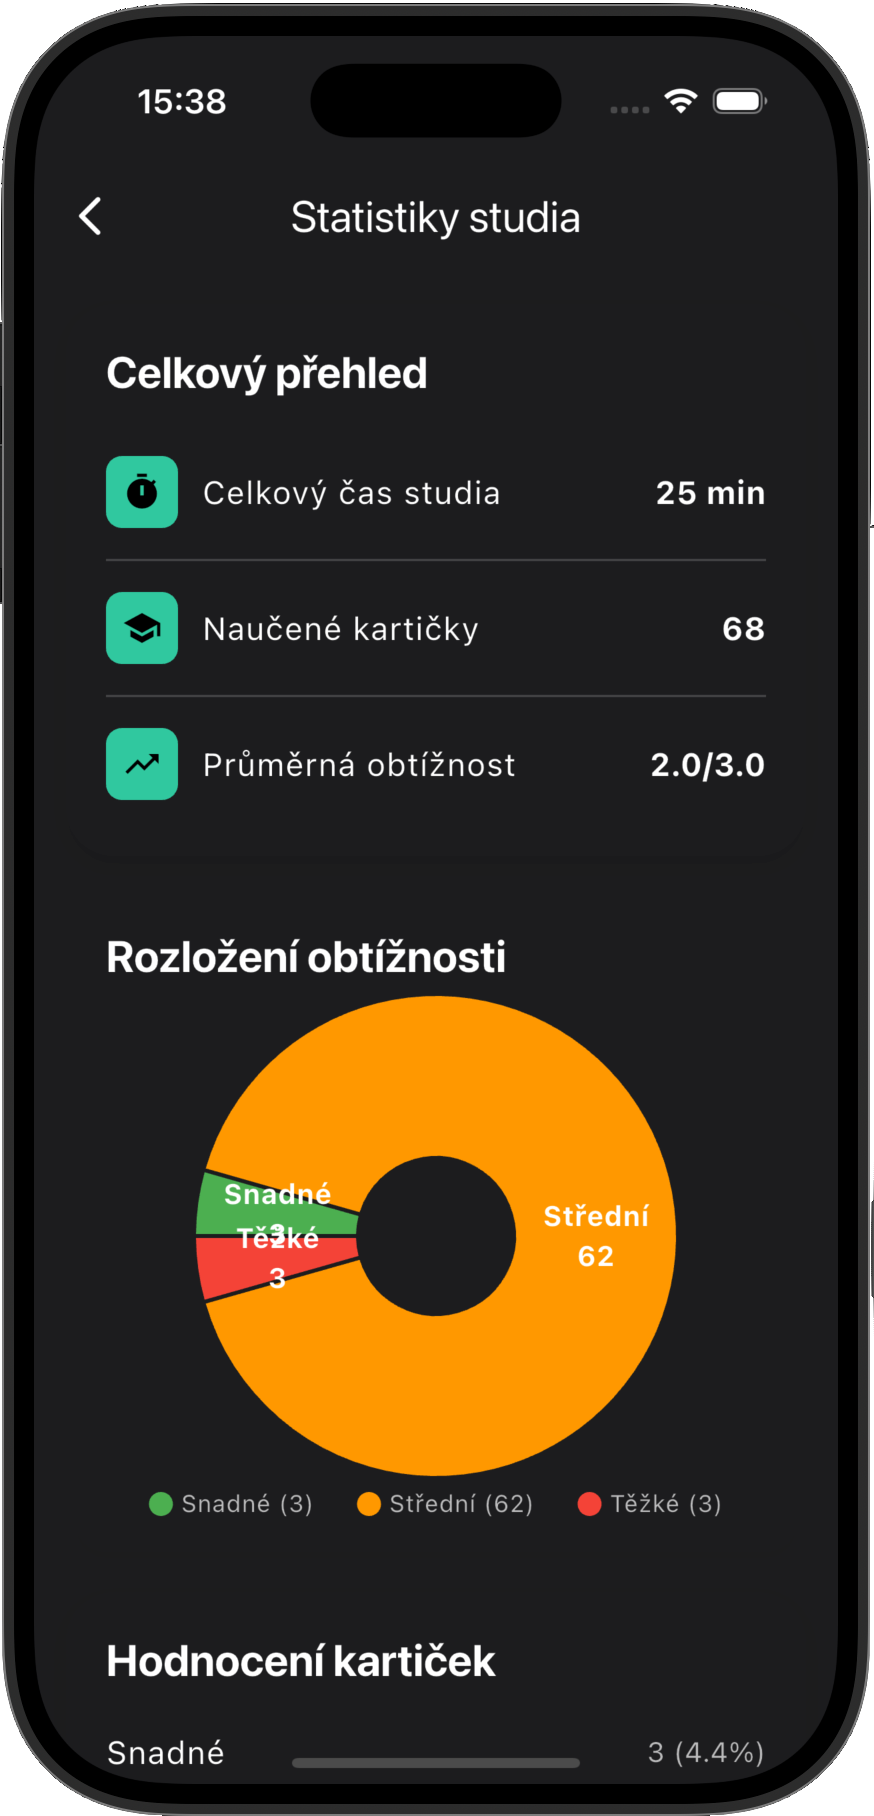
\includegraphics[width=\linewidth]{image/screen-statistics.png}
			\caption{Statistiky učení}
			\label{fig:screen-stats}
		\end{subfigure}
		\caption{Studijní a analytické obrazovky}
		\label{fig:study-screens}
	\end{figure}

	Implementované UI prvky:
	\begin{itemize}
		\item Responzivní layout pro různé velikosti obrazovek
		\item Adaptivní témata (světlý/tmavý režim)
		\item Plynulé animace a přechody
		\item Konzistentní typografie a barevné schéma
		\item Přístupné ovládací prvky
	\end{itemize}

	\section{Backend implementace}
	Backend aplikace jsem postavil na platformě Supabase, která poskytuje PostgreSQL databázi s realtime funkcionalitou. Implementace zahrnuje:

	\begin{itemize}
		\item Databázové schéma s tabulkami pro balíčky (decks), karty (cards) a záznamy o učení (study\_records)
		\item Row Level Security (RLS) politiky zajišťující přístup uživatelů pouze k vlastním datům
		\item Realtime synchronizaci pro okamžité aktualizace mezi zařízeními
		\item Optimalizované databázové dotazy a indexy pro rychlou odezvu
	\end{itemize}

	\begin{lstlisting}[style=Python, caption=Ukázka RLS politik]
-- Politika pro tabulku decks
CREATE POLICY "Uživatelé mohou číst pouze vlastní balíčky"
ON decks FOR SELECT
USING (auth.uid() = user_id);

-- Politika pro tabulku cards
CREATE POLICY "Uživatelé mohou číst karty z vlastních balíčků"
ON cards FOR SELECT
USING (
  EXISTS (
    SELECT 1 FROM decks
    WHERE decks.id = cards.deck_id
    AND decks.user_id = auth.uid()
  )
);
	\end{lstlisting}

	\section{Implementace Spaced Repetition}
	Implementace SuperMemo 2 algoritmu tvoří jádro učebního systému. Algoritmus je implementován v třídě SpacedRepetition, která poskytuje metody pro výpočet intervalů opakování na základě obtížnosti a počtu opakování.

	\begin{lstlisting}[style=Python, caption=Implementace algoritmu Spaced Repetition]
class SpacedRepetition {
  // Výpočet příštího intervalu opakování
  static DateTime calculateNextReview(
    DifficultyLevel difficulty,    // Obtížnost odpovědi
    int repetitionCount,           // Počet opakování
    DateTime lastReviewedAt,       // Poslední opakování
  ) {
    // Základní intervaly v hodinách
    final baseInterval = switch (difficulty) {
      DifficultyLevel.easy => 24 * 2.5,    // 2.5 dne
      DifficultyLevel.medium => 24,         // 1 den
      DifficultyLevel.hard => 6,            // 6 hodin
    };

    // Výpočet finálního intervalu
    final multiplier = (1.5 * repetitionCount).clamp(1.0, 30.0);
    final intervalHours = (baseInterval * multiplier).round();
    final randomFactor = 0.9 + (DateTime.now().millisecondsSinceEpoch % 200) / 1000;
    final finalIntervalHours = (intervalHours * randomFactor).round();

    return lastReviewedAt.add(Duration(hours: finalIntervalHours));
  }
}
	\end{lstlisting}

	\section{State Management}
	Pro správu stavu aplikace využívám Riverpod, který poskytuje typově bezpečný a deklarativní přístup ke správě stavu. Následující ukázka demonstruje implementaci providerů pro správu balíčků a kartiček.

	\begin{lstlisting}[style=Python, caption=Implementace Riverpod providerů]
@riverpod
class CurrentDeckNotifier extends _$CurrentDeckNotifier {
  @override
  AsyncValue<DeckEntity?> build() => const AsyncValue.data(null);

  Future<void> loadDeck(String deckId) async {
    state = const AsyncValue.loading();
    try {
      final repository = ref.read(deckRepositoryProvider);
      final deck = await repository.getDeck(deckId);
      state = AsyncValue.data(deck);
    } catch (error, stack) {
      state = AsyncValue.error(error, stack);
    }
  }
}

@riverpod
Future<List<CardEntity>> cardList(
  CardListRef ref,
  String deckId,
) async {
  final repository = ref.read(cardRepositoryProvider);
  return repository.getCards(deckId);
}
	\end{lstlisting}

	\section{Offline funkcionalita}
	Implementace offline režimu je založena na lokální SQLite databázi.

	Klíčové aspekty offline funkcionality:
	\begin{itemize}
		\item Plnohodnotná práce bez připojení k internetu
		\item Automatická synchronizace při obnovení připojení
		\item Sofistikované řešení konfliktů
		\item Queue systém pro operace
		\item Garance konzistence dat
	\end{itemize}

	\begin{figure}[h]
		\centering
		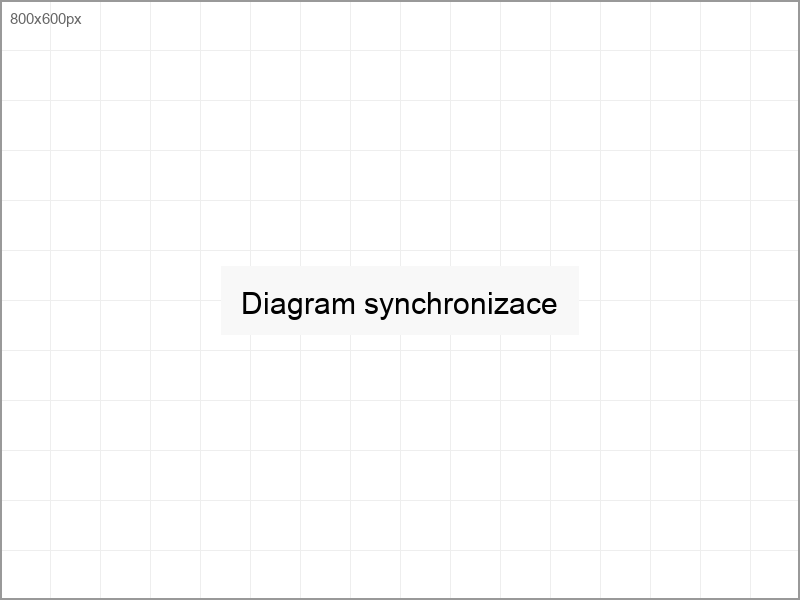
\includegraphics[width=0.8\linewidth]{image/diagram-sync.png}
		\caption{Diagram synchronizace dat}
		\label{fig:sync}
	\end{figure}

	Implementace offline funkcionality je založena na lokální SQLite databázi a systému front pro synchronizaci změn. Následující ukázka představuje implementaci synchronizačního manageru.

	\begin{lstlisting}[style=Python, caption=Implementace synchronizace]
class SyncManager {
  final SupabaseClient _client;    // Klient pro Supabase
  final LocalDatabase _localDb;    // Lokální databáze

  SyncManager(this._client, this._localDb);

  Future<void> synchronize() async {
    // Kontrola připojení k internetu
    if (!await _hasInternetConnection()) {
      debugPrint('Není připojení k internetu, synchronizace přeskočena');
      return;
    }

    try {
      // Proces synchronizace
      final localChanges = await _getLocalChanges();
      final serverChanges = await _getServerChanges();
      
      // Řešení konfliktů a aplikace změn
      final resolvedChanges = await _resolveConflicts(
        localChanges,
        serverChanges,
      );
      await _applyChangesToServer(resolvedChanges.serverUpdates);
      await _updateLocalDatabase(resolvedChanges.localUpdates);
      
      debugPrint('Synchronizace úspěšně dokončena');
    } catch (e) {
      debugPrint('Chyba při synchronizaci: $e');
      rethrow;
    }
  }
}
	\end{lstlisting}

\chapter{Výsledky a zhodnocení}
	\section{Splněné cíle}
	V rámci projektu se mi podařilo úspěšně implementovat všechny klíčové funkcionality a dosáhnout významných výsledků v oblasti mobilního vzdělávání.

	Dosažené milníky:
	\begin{itemize}
		\item Implementace algoritmu Spaced Repetition pro efektivní učení
		\item Realizace robustní offline funkcionality s automatickou synchronizací
		\item Vytvoření intuitivního uživatelského rozhraní s důrazem na UX
		\item Optimalizace výkonu aplikace a efektivní využití systémových zdrojů
		\item Implementace spolehlivého systému synchronizace mezi zařízeními
		\item Vytvoření komplexního systému pro správu učebních sad
		\item Zajištění bezpečného ukládání a přenosu dat
		\item Vytvoření solidního základu pro budoucí rozšíření
	\end{itemize}

	\section{Zhodnocení projektu}
	Projekt Repetito úspěšně naplnil stanovené cíle v oblasti mobilního vzdělávání a přinesl několik významných inovací.

	Hlavní přínosy projektu:
	\begin{itemize}
		\item Moderní technologický stack využívající Flutter, Riverpod a Supabase
		\item Efektivní implementace Spaced Repetition algoritmu pro optimální učení
		\item Robustní offline funkcionalita umožňující práci bez připojení k internetu
		\item Spolehlivá synchronizace dat mezi zařízeními
		\item Intuitivní uživatelské rozhraní s důrazem na UX
	\end{itemize}

	\section{Budoucí rozvoj}
	Na základě zkušeností z vývoje a zpětné vazby uživatelů byly identifikovány oblasti pro další rozvoj aplikace.

	Plánovaná vylepšení:
	\begin{itemize}
		\item Implementace nových typů učebního obsahu (audio, video)
		\item Rozšíření statistik učení o pokročilé analytické nástroje
		\item Optimalizace výkonu a snížení spotřeby baterie
		\item Přidání gamifikačních prvků pro zvýšení motivace
		\item Integrace umělé inteligence pro personalizaci učebního procesu
		\item Rozšíření možností sdílení a spolupráce mezi uživateli
	\end{itemize}

\chapter{Závěr}
	Mobilní aplikace Repetito představuje komplexní řešení pro efektivní učení pomocí metody spaced repetition. Projekt jsem rozdělil do tří hlavních částí: frontend aplikace vyvinuté ve frameworku Flutter, backend infrastruktury postavené na Supabase a sofistikovaného algoritmu pro optimalizaci učebního procesu.

	V aplikaci jsem úspěšně implementoval všechny klíčové funkcionality včetně správy učebních sad, offline režimu a synchronizace mezi zařízeními. Důraz jsem kladl na vytvoření intuitivního uživatelského rozhraní a optimalizaci výkonu. Využitím moderních technologií jako Riverpod pro správu stavu a Freezed pro generování kódu jsem zajistil robustní a udržitelnou architekturu.

	V průběhu vývoje jsem identifikoval možnosti dalšího rozvoje, které by mohly aplikaci posunout na další úroveň. Mezi hlavní plánovaná vylepšení patří implementace pokročilých statistik učení, integrace multimediálního obsahu a přidání gamifikačních prvků. Potenciál aplikace vidím nejen v individuálním vzdělávání, ale také ve školním prostředí nebo firemním vzdělávání.

	Zdrojový kód projektu je dostupný na GitHubu (\url{https://github.com/deathfrost12/repetito}).

\chapter*{Seznam použitých informačních zdrojů}
\addcontentsline{toc}{chapter}{Seznam použitých informačních zdrojů}

[1] Flutter Team. \textit{Flutter Documentation} [Online]. 2024 [cit. 2024-01-15]. Dostupné z: \url{https://flutter.dev/docs}

[2] Supabase Team. \textit{Supabase Documentation} [Online]. 2024 [cit. 2024-01-15]. Dostupné z: \url{https://supabase.com/docs}

[3] Remi Rousselet. \textit{Riverpod Documentation} [Online]. 2024 [cit. 2024-01-15]. Dostupné z: \url{https://riverpod.dev/docs}

[4] P. Wozniak. \textit{SuperMemo 2: An algorithm for intelligent learning} [Online]. 1998 [cit. 2024-01-15].

[5] Google. \textit{Material Design} [Online]. 2024 [cit. 2024-01-15]. Dostupné z: \url{https://m3.material.io/}

\end{document}